% Schematic of the measurement (a) and of the inference (b). Compile with pdflatex to fig_schematic.pdf.
\documentclass[border=2pt]{standalone}
\usepackage{amsmath,amssymb}
\usepackage{tikz}
\usetikzlibrary{arrows.meta,positioning,calc,shapes.geometric,fit,backgrounds}
\begin{document}
\footnotesize
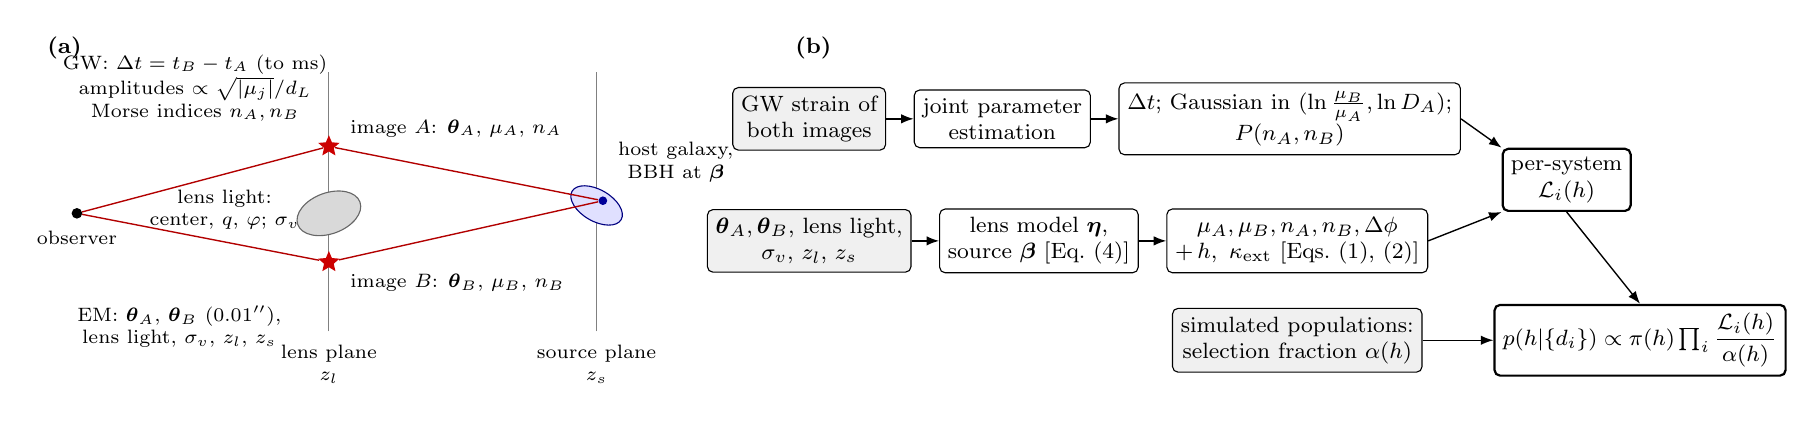
\begin{tikzpicture}[x=1cm,y=1cm,
  box/.style={draw,rounded corners=2pt,align=center,inner sep=3pt,font=\footnotesize,fill=white},
  data/.style={box,fill=black!6},
  res/.style={box,thick},
  arr/.style={-{Latex[length=1.6mm]},line width=0.5pt},
  lab/.style={font=\scriptsize,align=center}]
% ---------------------------------------------------------------- (a) geometry
\begin{scope}[shift={(0,0)}]
\node[font=\footnotesize\bfseries,anchor=west] at (-0.5,3.0) {(a)};
% observer
\node[draw,circle,inner sep=1.2pt,fill=black] (obs) at (0,0.9) {};
\node[lab,below=1pt of obs] {observer};
% lens plane
\draw[black!50] (3.2,-0.6) -- (3.2,2.7);
\node[lab,anchor=north] at (3.2,-0.65) {lens plane\\$z_l$};
\draw[fill=black!15,draw=black!60,rotate around={20:(3.2,0.9)}] (3.2,0.9) ellipse (0.42 and 0.26);
\node[lab,anchor=east] at (2.95,0.95) {lens light:\\center, $q$, $\varphi$; $\sigma_v$};
% images
\node[star,star points=5,star point ratio=2.2,fill=red!80!black,inner sep=1.3pt] (A) at (3.2,1.75) {};
\node[star,star points=5,star point ratio=2.2,fill=red!80!black,inner sep=1.3pt] (B) at (3.2,0.28) {};
\node[lab,anchor=west] at (3.35,1.98) {image $A$: $\boldsymbol\theta_A$, $\mu_A$, $n_A$};
\node[lab,anchor=west] at (3.35,0.02) {image $B$: $\boldsymbol\theta_B$, $\mu_B$, $n_B$};
% source plane
\draw[black!50] (6.6,-0.6) -- (6.6,2.7);
\node[lab,anchor=north] at (6.6,-0.65) {source plane\\$z_s$};
\draw[fill=blue!12,draw=blue!50!black,rotate around={-30:(6.6,1.0)}] (6.6,1.0) ellipse (0.36 and 0.2);
\node[fill=blue!60!black,circle,inner sep=1.1pt] (S) at (6.68,1.06) {};
\node[lab,anchor=west] at (6.75,1.55) {host galaxy,\\ BBH at $\boldsymbol\beta$};
% rays
\draw[red!70!black,line width=0.5pt] (S) -- (A) -- (obs);
\draw[red!70!black,line width=0.5pt] (S) -- (B) -- (obs);
% GW observables
\node[lab,anchor=south] at (1.5,1.95) {GW: $\Delta t=t_B-t_A$ (to ms)\\ amplitudes $\propto\sqrt{|\mu_j|}/d_L$\\ Morse indices $n_A,n_B$};
\node[lab,anchor=north] at (1.3,-0.15) {EM: $\boldsymbol\theta_A$, $\boldsymbol\theta_B$ (0.01$''$),\\ lens light, $\sigma_v$, $z_l$, $z_s$};
\end{scope}
% ---------------------------------------------------------------- (b) inference
\begin{scope}[shift={(9.3,0)}]
\node[font=\footnotesize\bfseries,anchor=west] at (-0.3,3.0) {(b)};
\node[data] (gw) at (0,2.1) {GW strain of\\ both images};
\node[box,right=0.35 of gw] (pe) {joint parameter\\ estimation};
\node[box,right=0.35 of pe] (gws) {$\Delta t$;\ Gaussian in $(\ln\frac{\mu_B}{\mu_A},\ln D_A)$;\\ $P(n_A,n_B)$};
\node[data] (em) at (0,0.55) {$\boldsymbol\theta_A,\boldsymbol\theta_B$, lens light,\\ $\sigma_v$, $z_l$, $z_s$};
\node[box,right=0.35 of em] (lens) {lens model $\boldsymbol\eta$,\\ source $\boldsymbol\beta$ [Eq.~(4)]};
\node[box,right=0.35 of lens] (pred) {$\mu_A,\mu_B,n_A,n_B,\Delta\phi$\\ $+\,h,\ \kappa_{\rm ext}$ [Eqs.~(1), (2)]};
\node[res] (post) at ($(gws.east)!0.5!(pred.east)+(1.55,0)$) {per-system\\ $\mathcal L_i(h)$};
\node[data] (pop) at ($(pred.south)+(0,-0.85)$) {simulated populations:\\ selection fraction $\alpha(h)$};
\node[res,right=0.9 of pop] (comb) {$p(h|\{d_i\})\propto\pi(h)\prod_i\dfrac{\mathcal L_i(h)}{\alpha(h)}$};
\draw[arr] (gw) -- (pe);
\draw[arr] (pe) -- (gws);
\draw[arr] (em) -- (lens);
\draw[arr] (lens) -- (pred);
\draw[arr] (gws.east) -- (post.north west);
\draw[arr] (pred.east) -- (post.south west);
\draw[arr] (post.south) -- (comb.north);
\draw[arr] (pop) -- (comb);
\end{scope}
\end{tikzpicture}
\end{document}
